%!TEX root = guide2.0.tex

% \section{Summary}\label{sec:PyMCObjects}
Bayesian inference begins with specification of a probability model relating unknown variables to data. PyMC provides three basic building blocks for Bayesian probability models: \code{Stochastic}, \code{Deterministic} and \code{Potential}.

A \code{Stochastic} object represents a variable whose value is not completely determined by its parents, and a \code{Deterministic} object represents a variable that is entirely determined by its parents. In object-oriented programming parlance, \code{Stochastic} and \code{Deterministic} are subclasses of the \code{Variable} class, which only serves as a template for other classes and is never actually implemented in models.

The third basic class, \code{Potential}, represents `factor potentials' (\cite{dawidmarkov,Jordan:2004p5439}), which are \emph{not} variables but simply terms and/or constraints that are multiplied into joint distributions to modify them. \code{Potential} and \code{Variable} are subclasses of \code{Node}.

% TODO: Need a better description of what a Potential is. Given the description of Stochastic and Deterministic we have given, its not clear where Potential fits in, as it classifies the world into 2 things -- completely determined by parents and not.

% PyMC also provides container classes for variables to make it easier to program of certain dependency situations, such as when a variable is defined by its dependence on an entire Markov chain.

\medskip
PyMC probability models are simply linked groups of \code{Stochastic}, \code{Deterministic} and \code{Potential} objects. These objects have very limited awareness of the models in which they are embedded and do not themselves possess methods for updating their values in fitting algorithms. Objects responsible for fitting probability models are described in chapter \ref{chap:modelfitting}.


\hypertarget{stochastic}{}
\section[The Stochastic class]{The \code{Stochastic} class}
\label{stochastic}
\pdfbookmark[0]{The Stochastic class}{stochastic}

A stochastic variable has the following primary attributes:
\begin{description}
    \item[\code{value}:] The variable's current value.
    \item[\code{logp}:] The log-probability of the variable's current value given the values of its parents.
\end{description}
A stochastic variable can optionally be endowed with a method called \code{\bfseries random}, which draws a value for the variable given the values of its parents\footnote{Note that the \code{random} method does not provide a Gibbs sample unless the variable has no children.}. Stochastic objects have the following additional attributes that are generally specified automatically, and only overridden under particular circumstances:
\begin{description}
    \item[\code{parents}:] A dictionary containing the variable's parents. The keys of the dictionary correspond to the names assigned to the variable's parents by the variable, and the values correspond to the actual parents. For example, the keys of $s$'s parents dictionary in model (\ref{disastermodel}) would be \code{'t_l'} and \code{'t_h'}. Thanks to Python's dynamic typing, the actual parents (\emph{i.e.} the values of the dictionary) may be of any class or type.
    \item[\code{children}:] A set containing the variable's children.
    \item[\code{extended_parents}:] A set containing all the stochastic variables on which the variable depends either directly or via a sequence of deterministic variables. If the value of any of these variables changes, the variable will need to recompute its log-probability.
    \item[\code{extended_children}:] A set containing all the stochastic variables and potentials that depend on the variable either directly or via a sequence of deterministic variables. If the variable's value changes, all of these variables will need to recompute their log-probabilities.
    % \item[\code{coparents}:] A set containing all the stochastic variables that share extended children with the variable.
    % \item[\code{moral_neighbors}:] A set containing the union of the variable's extended parents, extended children and coparents, with Potential objects removed.
    % \item[\code{markov_blanket}:] A set containing self and self's moral neighbors.
    \item[\code{observed}:] A flag (boolean) indicating whether the variable's value has been observed (is fixed).
    \item[\code{dtype}:] A NumPy dtype object (such as \code{numpy.int}) that specifies the type of the variable's value to fitting methods. If this is \code{None} (default) then no type is enforced.
    % \item[\code{__name__}:] The name of the variable, should be unique.
    %    \item[\code{__doc__}:] The docstring of the variable.
\end{description}

\subsection{Creation of stochastic variables}
There are three main ways to create stochastic variables, called the \textbf{automatic}, \textbf{decorator}, and \textbf{direct} interfaces.

\begin{description}
    \item[Automatic] Stochastic variables with standard distributions provided by PyMC (see chapter \ref{chap:distributions}) can be created in a single line using special subclasses of \code{Stochastic}. For example, the uniformly-distributed discrete variable $s$ in (\ref{disastermodel}) could be created using the automatic interface as follows:
\begin{verbatim}
    s = DiscreteUniform('s', 1851, 1962, value=1900)
\end{verbatim}

    In addition to the classes in chapter \ref{chap:distributions}, \code{scipy.stats.distributions}' random variable classes are wrapped as \code{Stochastic} subclasses if SciPy is installed. These distributions are in the submodule \code{pymc.SciPyDistributions}.

    Users can call the class factory \code{stochastic_from_dist} to produce \code{Stochastic} subclasses of their own from probability distributions not included with PyMC.%  These classes' init methods take the following arguments:
    % \begin{description}
    %     \item[\code{name}:] The name of the variable.
    %     \item[\code{value}:] An initial value for the variable.
    %     \item[\code{parents}:] Keyword arguments specifying the parents of the variable.
    %     \item[\code{observed} (optional)]
    %     \item[\code{doc} (optional):] The docstring of the variable.
    %     \item[\code{verbose} (optional):] An integer from 0 to 3.
    %     \item[\code{trace} (optional):] A boolean indicating whether a trace should be kept for this variable in Monte Carlo fitting methods.
    %     \item[\code{cache_depth}:] See section \ref{sec:caching}.
    % \end{description}


    \item[Decorator] Uniformly-distributed discrete stochastic variable $s$ in (\ref{disastermodel}) could alternatively be created from a function that computes its log-probability as follows:
\begin{verbatim}
@stochastic(dtype=int)
def s(value=1900, t_l=1851, t_h=1962):
    """The switchpoint for the rate of disaster occurrence."""
    if value > t_h or value < t_l:
        # Invalid values
        return -numpy.inf
    else:
        # Uniform log-likelihood
        return -numpy.log(t_h - t_l + 1)
\end{verbatim}
Note that this is a simple Python function preceded by a Python expression called a \textbf{decorator}, here called \code{@stochastic}. Generally, decorators enhance functions with additional properties or functionality. The \code{Stochastic} object produced by the \code{@stochastic} decorator will evaluate its log-probability using the function $s$. The \code{value} argument, which is required, provides an initial value for the variable. The remaining arguments will be assigned as parents of $s$ (\emph{i.e.} they will populate the \code{parents} dictionary).

To emphasize, the Python function decorated by \texttt{@stochastic} should compute the \emph{log}-density or \emph{log}-probability of the variable. That is why the return value in the example above is $-\log(t_h-t_l+1)$ rather than $1/(t_h-t_l+1)$.

The \code{value} and parents of stochastic variables may be any objects, provided the log-probability function returns a real number (\code{float}). PyMC and SciPy both provide implementations of several standard probability distributions that may be helpful for creating custom stochastic variables. Based on informal comparison using version 2.0, the distributions in PyMC tend to be approximately an order of magnitude faster than their counterparts in SciPy (using version 0.7). See \href{http://code.google.com/p/pymc/wiki/Benchmarks}{the wiki page on benchmarks}  There are two reasons:

    The decorator \code{stochastic} can take several arguments:
    \begin{itemize}
        \item A flag called \code{trace}, which signals to \code{MCMC} instances whether an MCMC trace should be kept for this variable. \code{@stochastic(trace = False)} would turn tracing off. Defaults to \code{True}.
        \item A flag called \code{plot}, which signals to \code{MCMC} instances whether summary plots should be produced for this variable. Defaults to \code{True}.
        \item An integer-valued argument called \code{verbose} that controls the amount of output the variable prints to the screen. The default is $0$, no output; the maximum value is $3$.
        \item A Numpy datatype called \code{dtype}. Decorating a log-probability function with \code{@stochastic(dtype=int)} would produce a discrete random variable. Such a variable will cast its value to either an integer or an array of integers. The default dtype is \code{float}.
    \end{itemize}

    The decorator interface has a slightly more complex implementation which allows you to specify a \code{random} method for sampling the stochastic variable's value conditional on its parents.
    \begin{verbatim}
@stochastic(dtype=int)
def s(value=1900, t_l=1851, t_h=1962):
    """The switchpoint for the rate of disaster occurrence."""

    def logp(value, t_l, t_h):
        if value > t_h or value < t_l:
            return -Inf
        else:
            return -log(t_h - t_l + 1)

    def random(t_l, t_h):
        return np.round( (t_l - t_h) * random() ) + t_l

    \end{verbatim}
The stochastic variable again gets its name, docstring and parents from function $s$, but in this case it will evaluate its log-probability using the \code{logp} function. The \code{random} function will be used when \code{s.random()} is called. Note that \code{random} doesn't take a \code{value} argument, as it generates values itself. The optional \code{rseed} variable provides a seed for the random number generator. The stochastic's \code{value} argument is optional when a \code{random} method is provided; if no initial value is provided, it will be drawn automatically using the \code{random} method.

    \item[Direct] It's possible to instantiate \code{Stochastic} directly:
\begin{verbatim}
def s_logp(value, t_l, t_h):
    if value > t_h or value < t_l:
        return -Inf
    else:
        return -log(t_h - t_l + 1)

def s_rand(t_l, t_h):
    return np.round( (t_l - t_h) * random() ) + t_l

s = Stochastic( logp = s_logp,
                doc = 'The switchpoint for the rate of disaster occurrence.',
                name = 's',
                parents = {'t_l': 1851, 't_h': 1962},
                random = s_rand,
                trace = True,
                value = 1900,
                dtype=int,
                rseed = 1.,
                observed = False,
                cache_depth = 2,
                plot=True,
                verbose = 0)
\end{verbatim}
Notice that the log-probability and random variate functions are specified externally and passed to \code{Stochastic} as arguments. This is a rather awkward way to instantiate a stochastic variable; consequently, such implementations should be rare.

\end{description}

\begin{center}
\begin{boxedminipage}{.9\textwidth}
\subsection{Don't update stochastic variables' values in-place}


\code{Stochastic} objects' values should not be updated in-place. This confuses PyMC's caching scheme and corrupts the process used for accepting or rejecting proposed values in the MCMC algorithm. The only way a stochastic variable's value should be updated is using statements of the following form:
\begin{verbatim}
    A.value = new_value
\end{verbatim}
The following are in-place updates and should \emph{never} be used:
\begin{itemize}
    \item \code{A.value += 3}
    \item \code{A.value[2,1] = 5}
    \item \code{A.value.attribute = new_attribute_value}.
\end{itemize}

This restriction becomes onerous if a step method proposes values for the elements of an array-valued variable separately. In this case, it may be preferable to partition the variable into several scalar-valued variables stored in an array or list.
\end{boxedminipage}
\end{center}

\hypertarget{data}{}
\section{Data} \label{data}
\pdfbookmark[0]{Data}{data}

Although the data are modelled with statistical distributions, their values should be treated as immutable (since they have been observed). Data are represented by \code{Stochastic} objects whose \code{observed} attribute is set to \code{True}. If a stochastic variable's \code{observed} flag is \code{True}, its value cannot be changed, and it won't be sampled by the fitting method..

\subsection{Declaring stochastic variables to be data}

In each interface, an optional keyword argument \code{observed} can be set to \code{True}. In the decorator interface, this argument is added to the \code{@stochastic} decorator:

\begin{verbatim}
@stochastic(observed=True)
\end{verbatim}

In the other interfaces, the \code{observed=True} argument is added to the instantiation of the \code{Stochastic}, or its subclass:

\begin{verbatim}
	x = Binomial('x', n=n, p=p, observed=True)
\end{verbatim}

Alternatively, in the decorator interface only, a \code{Stochastic} object's \code{observed} flag can be set to true by stacking an \code{@observed} decorator on top of the \code{@stochastic} decorator:
\begin{verbatim}
@observed
@stochastic(dtype=int)
\end{verbatim}

\hypertarget{deterministic}{}
\section[The Deterministic class]{The \code{Deterministic} class}
\label{deterministic}
\pdfbookmark[0]{The Deterministic class}{deterministic}

The \code{Deterministic} class represents variables whose values are completely determined by the values of their parents. For example, in model (\ref{disastermodel}), $r$ is a \code{deterministic} variable. Recall it was defined by
\begin{eqnarray*}
    r_t=\left\{\begin{array}{ll}
        e & t\le s\\ l & t>s
        \end{array}\right.,
\end{eqnarray*}
so $r$'s value can be computed exactly from the values of its parents $e$, $l$ and $s$.

A \code{deterministic} variable's most important attribute is \code{\bfseries value}, which gives the current value of the variable given the values of its parents. Like \code{Stochastic}'s \code{logp} attribute, this attribute is computed on-demand and cached for efficiency.

A Deterministic variable has the following additional attributes:
\begin{description}
    \item[\code{parents}:] A dictionary containing the variable's parents. The keys of the dictionary correspond to the names assigned to the variable's parents by the variable, and the values correspond to the actual parents. Thanks to Python's dynamic typing, parents may be of any class or type.
    \item[\code{children}:] A set containing the variable's children, which must be nodes.
    % \item[\code{__name__}:] The name of the variable, should be unique.
    %     \item[\code{__doc__}:] The docstring of the variable.
\end{description}
Deterministic variables have no methods.


\subsection{Creation of deterministic variables}
Deterministic variables are less complicated than stochastic variables, and have similar \textbf{automatic}, \textbf{decorator}, and \textbf{direct} interfaces:
\begin{description}
   \item[Automatic] A handful of common functions have been wrapped in Deterministic objects. These are brief enough to list:
   \begin{description}
      \item[\code{LinearCombination}:] Has two parents $x$ and $y$, both of which must be iterable (\emph{i.e.} vector-valued). This function returns:
      \[
      \sum_i x_i^T y_i.
      \]
      \item[\code{Index}:] Has three parents $x$, $y$ and \code{index}. $x$ and $y$ must be iterables, \code{index} must be valued as an integer. Index returns the dot product of $x$ and $y$ for the elements specified by \texttt{index}:
      \[
      x[\mathtt{index}]^T y[\mathtt{index}].
      \]
      \code{Index} is useful for implementing dynamic models, in which the parent-child connections change.
      \item[\code{Lambda}:] Converts an anonymous function (in Python, called \textbf{lambda functions}) to a \code{Deterministic} instance on a single line.
      \item[\code{CompletedDirichlet}:] PyMC represents Dirichlet variables of length $k$ by the first $k-1$ elements; since they must sum to 1, the $k^{th}$ element is determined by the others. \code{CompletedDirichlet} appends the $k^{th}$ element to the value of its parent $D$.
      \item[\code{Logit}, \code{InvLogit}, \code{StukelLogit}, \code{StukelInvLogit}:] Various common link functions for generalized linear models.
   \end{description}
   It's a good idea to use these classes when feasible, because certain fitting methods (Gibbs step methods in particular) implicitly know how to take them into account.

    \item[Decorator] A deterministic variable can be created via a decorator in a way very similar to \code{Stochastic}'s decorator interface:
\begin{verbatim}
@deterministic
def r(switchpoint = s, early_rate = e, late_rate = l):
    """The rate of disaster occurrence."""
    value = zeros(N)
    value[:switchpoint] = early_rate
    value[switchpoint:] = late_rate
    return value
\end{verbatim}
Notice that rather than returning the log-probability, as is the case for \code{Stochastic} objects, the function returns the value of the deterministic object, given its parents. This return value may be of any type, as is suitable for the problem at hand. Also notice that, unlike for \code{Stochastic} objects, there is no \code{value} argument passed, since the value is calculated deterministically by the function itself. Arguments' keys and values are converted into a parent dictionary as with \code{Stochastic}'s short interface. The \code{deterministic} decorator can take \code{trace}, \code{verbose} and \code{plot} arguments, like the \code{stochastic} decorator\footnote{Note that deterministic variables have no \code{observed} flag. If a deterministic variable's value were known, its parents would be restricted to the inverse image of that value under the deterministic variable's evaluation function. This usage would be extremely difficult to support in general, but it can be implemented for particular applications at the \code{StepMethod} level.}.

Of course, since deterministic nodes are not expected to generate random variates, the longer implementation of the decorator interface available to \code{Stochastic} objects is not relevant here.

    \item[Direct] Deterministic objects can also be instantiated directly, by passing the evaluation function to the \texttt{Deterministic} class as an argument:
\begin{verbatim}
def r_eval(switchpoint = s, early_rate = e, late_rate = l):
    value = zeros(N)
    value[:switchpoint] = early_rate
    value[switchpoint:] = late_rate
    return value

r = Deterministic(  eval = r_eval,
                    name = 'r',
                    parents = {'switchpoint': s, 'early_rate': e, 'late_rate': l}),
                    doc = 'The rate of disaster occurrence.',
                    trace = True,
                    verbose = 0,
                    dtype=float,
                    plot=False,
                    cache_depth = 2)
\end{verbatim}
\end{description}

\hypertarget{container}{}
\section{Containers} \label{container}
\pdfbookmark[0]{Containers}{container}

In some situations it would be inconvenient to assign a unique label to each parent of some variable. Consider $y$ in the following model:
\begin{align*}
    x_0 &\sim \textup N (0,\tau_x)\\
    x_{i+1}|x_i &\sim \textup{N}(x_i, \tau_x)\\
    &&i=0,\ldots, N-2\\
    y|x &\sim \textup N \left(\sum_{i=0}^{N-1}x_i^2,\tau_y\right)
\end{align*}
Here, $y$ depends on every element of the Markov chain $x$, but we wouldn't want to manually enter $N$ parent labels \code{`x_0'}, \code{`x_1'}, etc.

This situation can be handled naturally in PyMC:
\begin{verbatim}
x_0 = Normal(`x_0', mu=0, tau=1)

# Initialize array of stochastics
x = np.empty(N,dtype=object)
x[0] = x_0

# Loop over number of elements in N
for i in range(1,N):

   # Instantiate Normal stochastic, based on value of previous element in x
   x[i] = Normal(`x_%i' % i, mu=x[-1], tau=1)

@observed
@stochastic
def y(value = 1, mu = x, tau = 100):
    mu_sum = np.sum(mu**2)
    return normal_like(value, mu_sum, tau)
\end{verbatim}
PyMC automatically wraps list $x$ in an appropriate \code{Container} class. The  expression \code{`x_\%i' \% i} labels each \code{Normal} object in the container with the appropriate index $i$; so if \code{i=1}, the name of the corresponding element becomes \code{`x_1'}.

Containers, like variables, have an attribute called \code{value}. This attribute returns a copy of the (possibly nested) iterable that was passed into the container function, but with each variable inside replaced with its corresponding value.

Containers can currently be constructed from lists, tuples, dictionaries, Numpy arrays, modules, sets or any object with a \code{__dict__} attribute. Variables and non-variables can be freely mixed in these containers, and different types of containers can be nested\footnote{Nodes whose parents are containers make private shallow copies of those containers. This is done for technical reasons rather than to protect users from accidental misuse.}. Containers attempt to behave like the objects they wrap. All containers are subclasses of \code{ContainerBase}.

Containers have the following useful attributes in addition to \code{value}:
\begin{itemize}
    \item\code{variables}
    \item\code{stochastics}
    \item\code{potentials}
    \item\code{deterministics}
    \item\code{data_stochastics}
    \item\code{step_methods}.
\end{itemize}
Each of these attributes is a set containing all the objects of each type in a container, and within any containers in the container.


\hypertarget{potential}{}
\section[The Potential class]{The \code{Potential} class} \label{potential}
\pdfbookmark[0]{The Potential class}{potential}

% See the two examples here and the extended example below. Is that enough?

The joint density corresponding to model (\ref{disastermodel}) can be written as follows:
\begin{eqnarray*}
    p(D,s,l,e) = p(D|s,l,e) p(s) p(l) p(e).
\end{eqnarray*}
Each factor in the joint distribution is a proper, normalized probability distribution for one of the variables conditional on its parents. Such factors are contributed by \code{Stochastic} objects.

In some cases, it's nice to be able to modify the joint density by incorporating terms that don't correspond to probabilities of variables conditional on parents, for example:
\begin{eqnarray*}
    p(x_0, x_2, \ldots x_{N-1}) \propto \prod_{i=0}^{N-2} \psi_i(x_i, x_{i+1}).
\end{eqnarray*}


In other cases we may want to add probability terms to existing models. For example, suppose we want to constrain the difference between $e$ and $l$ in (\ref{disastermodel}) to be less than 1, so that the joint density becomes
\begin{eqnarray*}
    p(D,s,l,e) \propto p(D|s,l,e) p(s) p(l) p(e) I(|e-l|<1).
\end{eqnarray*}
It's possible to express this constraint by adding variables to the model, or by grouping $e$ and $l$ to form a vector-valued variable, but it's uncomfortable to do so.

Arbitrary factors such as $\psi$ and the indicator function $I(|e-l|<1)$ are
implemented by objects of class \code{Potential} (\cite{dawidmarkov} and
\cite{Jordan:2004p5439} call these terms `factor potentials'). Bayesian
hierarchical notation (cf model (\ref{disastermodel})) doesn't accomodate these
potentials. They are often used in cases where there is no natural dependence
hierarchy, such as the first example above (which is known as a Markov random
field). They are also useful for expressing `soft data'
\citep{Christakos:2002p5506} as in the second example above.


\bigskip
Potentials have one important attribute, \code{\bfseries logp}, the log of their current probability or probability density value given the values of their parents. The only other additional attribute of interest is \code{parents}, a dictionary containing the potential's parents. Potentials have no methods. They have no \code{trace} attribute, because they are not variables. They cannot serve as parents of variables (for the same reason), so they have no \code{children} attribute.

\subsection{An example of soft data}
The role of potentials can be confusing, so we will provide another example: we have a dataset $t$ consisting of the days on which several marked animals were recaptured. We believe that the probability $S$ that an animal is not recaptured on any given day can be explained by a covariate vector $x$. We model this situation as follows:
\begin{eqnarray*}
    t_i|S_i \sim \textup{Geometric}(S_i), & i=1\ldots N\\
    S_i = \textup{logit}^{-1}(\beta x_i), &i=1\ldots N\\
    \beta\sim \textup{N}(\mu_\beta, V_\beta).
\end{eqnarray*}
So far, so good. Now suppose we have some knowledge of other related experiments and we have a good idea of what $S$ will be independent of the value of $\beta$. It's not obvious how to work this `soft data', because as we've written the model $S$ is completely determined by $\beta$. There are three options within the strict Bayesian hierarchical framework:
\begin{itemize}
    \item Work the soft data into the prior on $\beta$.
    \item Incorporate the data from the previous experiments explicitly into the model.
    \item Refactor the model so that $S$ is at the bottom of the hierarchy, and assign the prior directly.
\end{itemize}

Factor potentials provide a convenient way to incorporate the soft data without the need for such major modifications. We can simply modify the joint distribution from
\begin{eqnarray*}
    p(t|S(x,\beta)) p(\beta)
\end{eqnarray*}
to
\begin{eqnarray*}
    \gamma(S) p(t|S(x,\beta)) p(\beta),
\end{eqnarray*}
where the value of $\gamma$ is large if $S$'s value is plausible (based on our external information) and small otherwise. We do not know the normalizing constant for the new distribution, but we don't need it to use most popular fitting algorithms. It's a good idea to check the induced priors on $S$ and $\beta$ for sanity. This can be done in PyMC by fitting the model with the data $t$ removed.

It's important to understand that $\gamma$ is not a variable, so it does not have a value. That means, among other things, there will be no $\gamma$ column in MCMC traces. $\gamma$ is simply an extra term that we are incorporating in the joint distribution.


\subsection[Creation of Potentials]{Creation of \code{Potentials}}
There are two ways to create potentials:
\begin{description}
    \item[Decorator] A potential can be created via a decorator in a way very similar to \code{Deterministic}'s decorator interface:
\begin{verbatim}
@potential
def psi_i(x_lo = x[i], x_hi = x[i+1]):
    """A pair potential"""
    return -(xlo - xhi)**2
\end{verbatim}
The function supplied should return the potential's current \emph{log}-probability or \emph{log}-density as a Numpy \code{float}. The \code{potential} decorator can take \code{verbose} and \code{cache_depth} arguments like the \code{stochastic} decorator.
    \item[Direct] The same potential could be created directly as follows:
\begin{verbatim}
def psi_i_logp(x_lo = x[i], x_hi = x[i+1]):
    return -(xlo - xhi)**2

psi_i = Potential(  logp = psi_i_logp,
                    name = 'psi_i',
                    parents = {'xlo': x[i], 'xhi': x[i+1]},
                    doc = 'A pair potential',
                    verbose = 0,
                    cache_depth = 2)
\end{verbatim}
\end{description}


\hypertarget{graphical}{}
\section{Graphing models} \label{graphical}
\pdfbookmark[0]{Graphing models}{graphical}

The function \code{graph} in \code{pymc.graph} draws graphical representations of \code{Model} (Chapter \ref{chap:modelfitting}) instances using GraphViz via the Python package PyDot (if they are installed). See \cite{dawidmarkov} and \cite{Jordan:2004p5439} for more discussion of useful information that can be read off of graphical models. Note that these authors do not consider deterministic variables.

The symbol for stochastic variables is an ellipse. Parent-child relationships are indicated by arrows. These arrows point from parent to child and are labeled with the names assigned to the parents by the children. PyMC's symbol for deterministic variables is a downward-pointing triangle. A graphical representation of model \ref{disastermodel} follows:
\begin{center}
    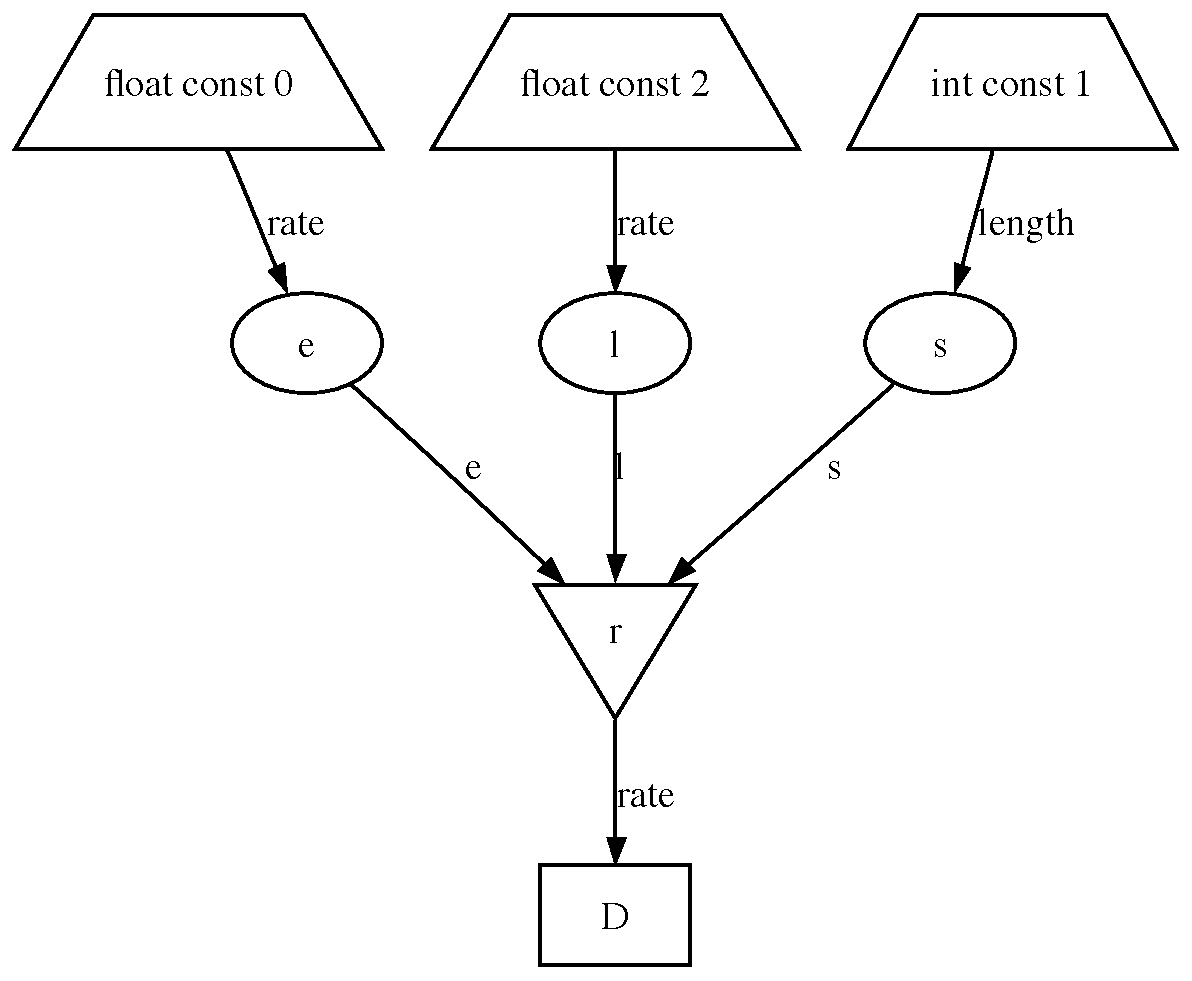
\epsfig{file=DisasterModel2.pdf, width=6cm}
\end{center}
$D$ is shaded because it is flagged as data.

% Note that if a deterministic variable has more than one child, its parents each inherit all of its children when it is made implicit:
% \begin{center}
%     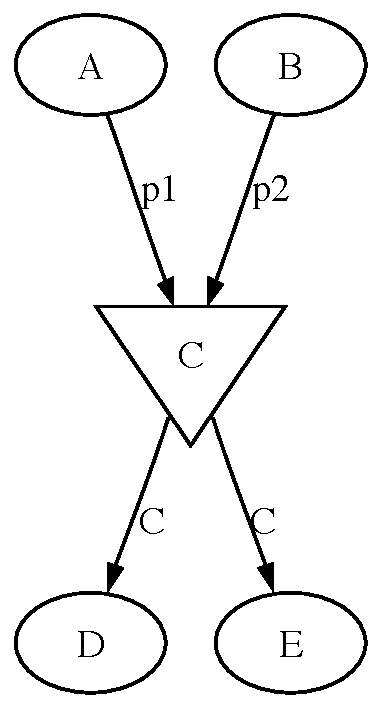
\epsfig{file=DeterministicPreInheritance.pdf, width=3.5cm} $\Rightarrow$ 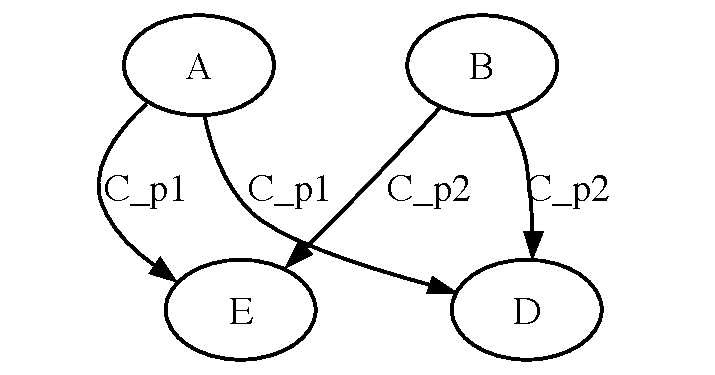
\epsfig{file=DeterministicPostInheritance.pdf, width=5cm}
% \end{center}
% These inherited children can be accessed via the \code{extended_children} attributes of the parents.

The symbol for factor potentials is a rectangle, as in the following model.
\begin{center}
    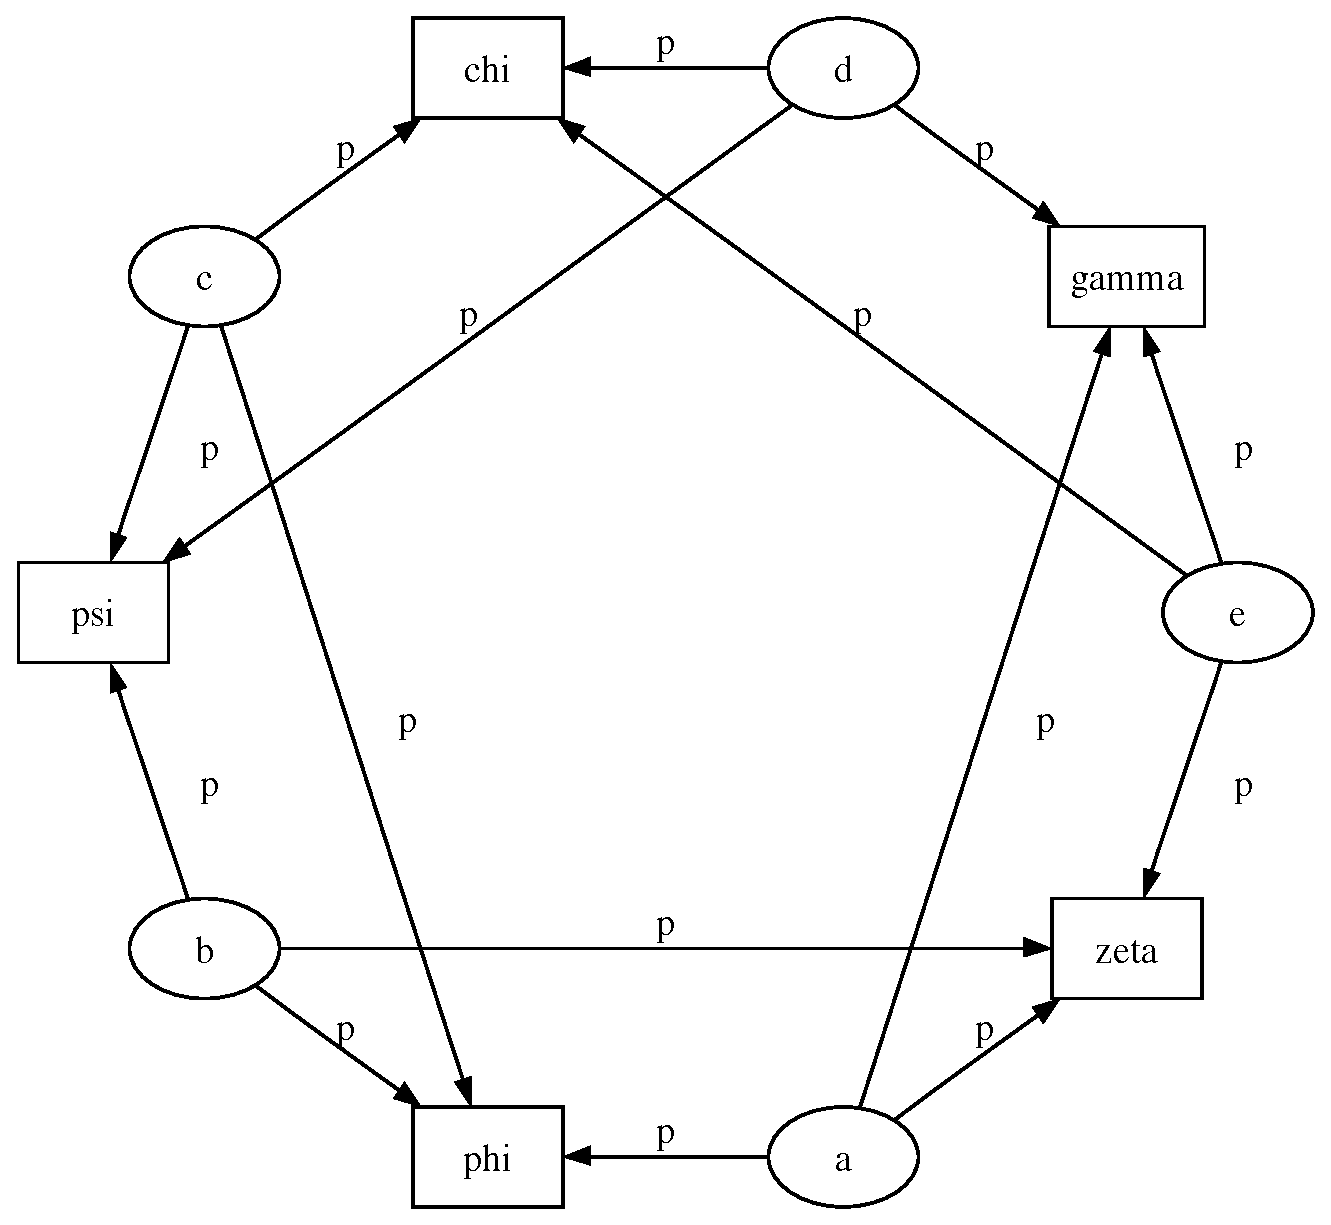
\epsfig{file=PotExample.pdf, width=10cm}
\end{center}
Factor potentials are usually associated with \emph{undirected} grahical models. In undirected representations, each parent of a potential is connected to every other parent by an undirected edge. The undirected representation of the model pictured above is much more compact:
\begin{center}
    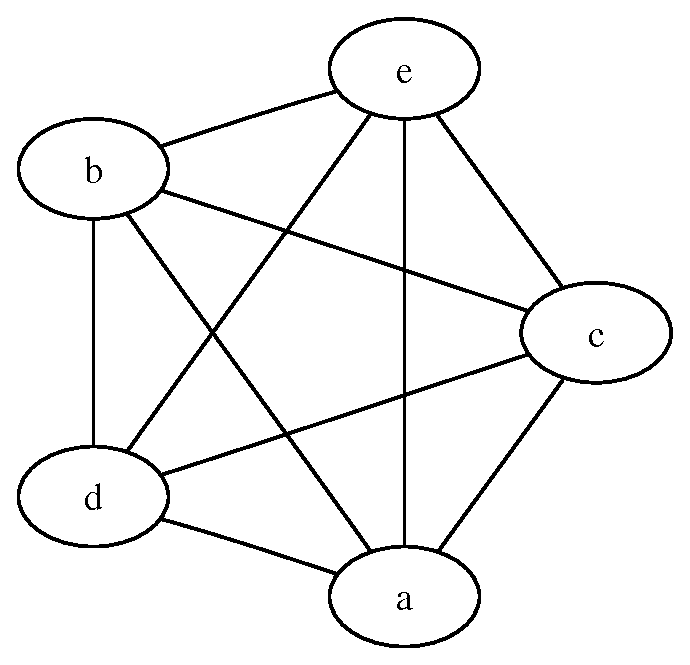
\epsfig{file=PotExampleCollapsed.pdf, width=5cm}
\end{center}
Directed or mixed graphical models can be represented in an undirected form by `moralizing', which is done by the function \code{pymc.graph.moral_graph}.


\section[Class LazyFunction and caching]{Class \code{LazyFunction}
and caching}
\label{sec:caching}
This section gives an overview of how PyMC computes log-probabilities. This is advanced information that is not required in order to use PyMC.

The \code{logp} attributes of stochastic variables and potentials and the \code{value} attributes of deterministic variables are wrappers for instances of class \code{LazyFunction}. Lazy functions are wrappers for ordinary Python functions. A lazy function \code{L} could be created from a function \code{fun} as follows:
\begin{verbatim}
L = LazyFunction(fun, arguments)
\end{verbatim}
The argument \code{arguments} is a dictionary container; \code{fun} must accept keyword arguments only. When \code{L}'s \code{get()} method is called, the return value is the same as the call
\begin{verbatim}
fun(**arguments.value)
\end{verbatim}
Note that no arguments need to be passed to \code{L.get}; lazy functions memorize their arguments.

Before calling \code{fun}, \code{L} will check the values of \code{arguments.variables} against an internal cache. This comparison is done \emph{by reference}, not by value, and this is part of the reason why stochastic variables' values cannot be updated in-place. If \code{arguments.variables}' values match a frame of the cache, the corresponding output value is returned and \code{fun} is not called. If a call to \code{fun} is needed, \code{arguments.variables}' values and the return value replace the oldest frame in the cache. The depth of the cache can be set using the optional init argument \code{cache_depth}, which defaults to 2.

Caching is helpful in MCMC, because variables' log-probabilities and values tend to be queried multiple times for the same parental value configuration. The default cache depth of 2 turns out to be most useful in Metropolis-Hastings-type algorithms involving proposed values that may be rejected.

Lazy functions are implemented in C using Pyrex, a language for writing Python extensions.
